\tocless\section{561. Array Partition I}
\label{algo:561}

\subsection*{Difficulty}
Easy

\subsection*{Tags}
String \& Array

\subsection*{Description}
Given an array of $2n$ integers, your task is to group these integers into n pairs of integer, say $(a_1, b_1), (a_2, b_2), \dots, (a_n, b_n)$ which makes sum of $min(a_i, b_i)$ for all $i$ from $1$ to $n$ as large as possible.

\begin{example}
\begin{multilinecode}
Input: [1, 4, 3, 2]
Output: 4

Explanation: n is 2, and the maximum sum of pairs is 4 = min(1, 2) + min(3, 4).
\end{multilinecode}
\end{example}

\textbf{Note}
\begin{itemize}
    \item $n$ is a positive integer, which is in the range of $[1, 10000]$.
    \item All the integers in the array will be in the range of $[-10000, 10000]$.
\end{itemize}

\subsection*{Analysis}
At first sight, you may wonder that what an easy problem it is. All we need to do is sort this array and fetch every other element from 0. In this manner, however, we get a time complexity of $O(n{\log}n)$, assuming that the number of array is $n$, because we have to sort the array. After that, we may think a linear method to calculate the sum.

Therefore, we use buckets $b[0..i..n]$ to store the elements. $x[i]$ is the element and $b[i]$ is the count of this element, because we notice that if the count of an element is odd, the remaining one element have to participate the comparison to next elements. Hence, we use a $flag$ to record whether the count of last element is odd or even. If flag is odd, then in the next element, we have
\begin{multilinecode}
sum[i + 1] = sum[i] + (x[i] + ((b[i + 1] - 1) / 2) * x[i + 1]
\end{multilinecode}

because $x[i + 1]$ has to contribute one element to compare with $x[i]$. And when flag is even, we have
\begin{multilinecode}
sum[i + 1] = sum[i] + (x[i] + (b[i + 1] / 2) * x[i + 1]
\end{multilinecode}
And then we need to check $b[x + 1]$ to set the flag.

The cases are shown in the figure below:

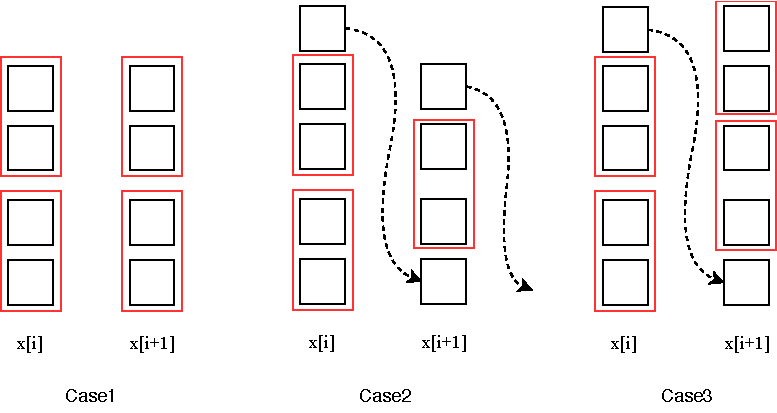
\includegraphics{figs/algo_561_1}

\begin{itemize}
    \item Time Complexity: $\mathcal{O}(n)$
    \item Space Complexity: $\mathcal{O}(n)$
\end{itemize}

\subsection*{Solution}
\subsubsection*{C}
\begin{minted}[framesep=2mm,
baselinestretch=1.2,
bgcolor=codebackground,
fontsize=\footnotesize,
linenos]{c}
int arrayPairSum(int* nums, int numsSize) {
    int distinct_nums[20001] = { 0 };
    for (int i = 0; i < numsSize; ++i) {
        ++distinct_nums[nums[i] + 10000];
    }
    int result = 0;
    // flag to record the count of element is odd or even
    int flag = 0;
    // previous element
    int prev;
    for (int i = 0, x = -10000; i <= 20000; ++i, ++x) {
        int count = distinct_nums[i];
        if (count == 0) continue;
        // last count is even
        if (flag == 0) {
            result += x * (count >> 1);
            // remaining element
            if ((count & 1) == 1) {
                flag = 1;
                prev = x;
            } else {
                flag = 0;
            }
        } else {  // last count is odd
            int a = count & 1;
            result += x * ((count - 1) >> 1) + prev;
            // remaining element
            if ((count & 1) == 0) {
                flag = 1;
                prev = x;
            } else {
                flag = 0;
            }
        }
    }
    return result;
}
\end{minted}

\newpage
